\newpage
\subsection{Mechanical Design} \label{Mechanical_Design}
\label{sec:mechanical-design}

\subsubsection{Structure}

\begin{figure}[H]
	\centering 
	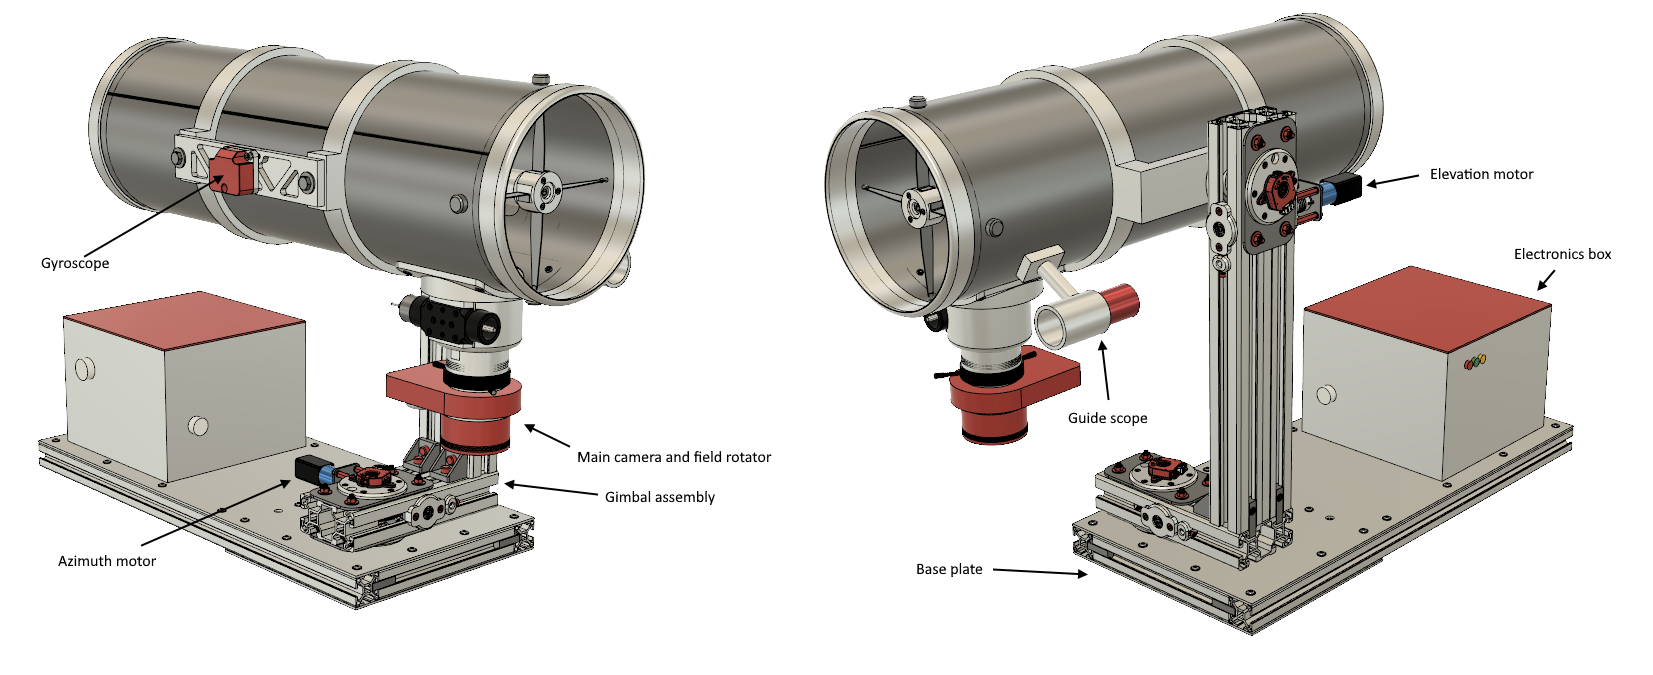
\includegraphics[scale=0.4]{4-experiment-design/img/mechanical/iso1.png}
	\caption{Experiment module overview.}
	\label{fig::mechanical::iso1}
\end{figure}

\label{sec:4.4.1}
The experiment has three components that are placed inside the gondola:
\begin{itemize}
  \item Mounting plate    
  \item Electronics box
  \item Gimbal and telescope assembly
\end{itemize}

We require the gimbal to be placed at the edge of the gondola so that the telescope is capable of performing its required range of motion for observing astronomical targets.



\subsubsection{Mounting plate}

The mounting plate is constructed from aluminium sheet and 30 mm aluminium extrusions. It is affixed to the gondola mounting rails using M6 t-head bolts and angle brackets. 

\subsubsection{Electronics box}
\label{sec:4.4.2}

The electronics box has a dimension 20x20x15 cm which is placed directly inside the gondola, see figure \ref{fig::mechanical::ebox}. The box is made of aluminium side plates with a layer of polystyrene on the inside. All electronics are mounted on standoffs 

\begin{figure}[H]
	\centering 
	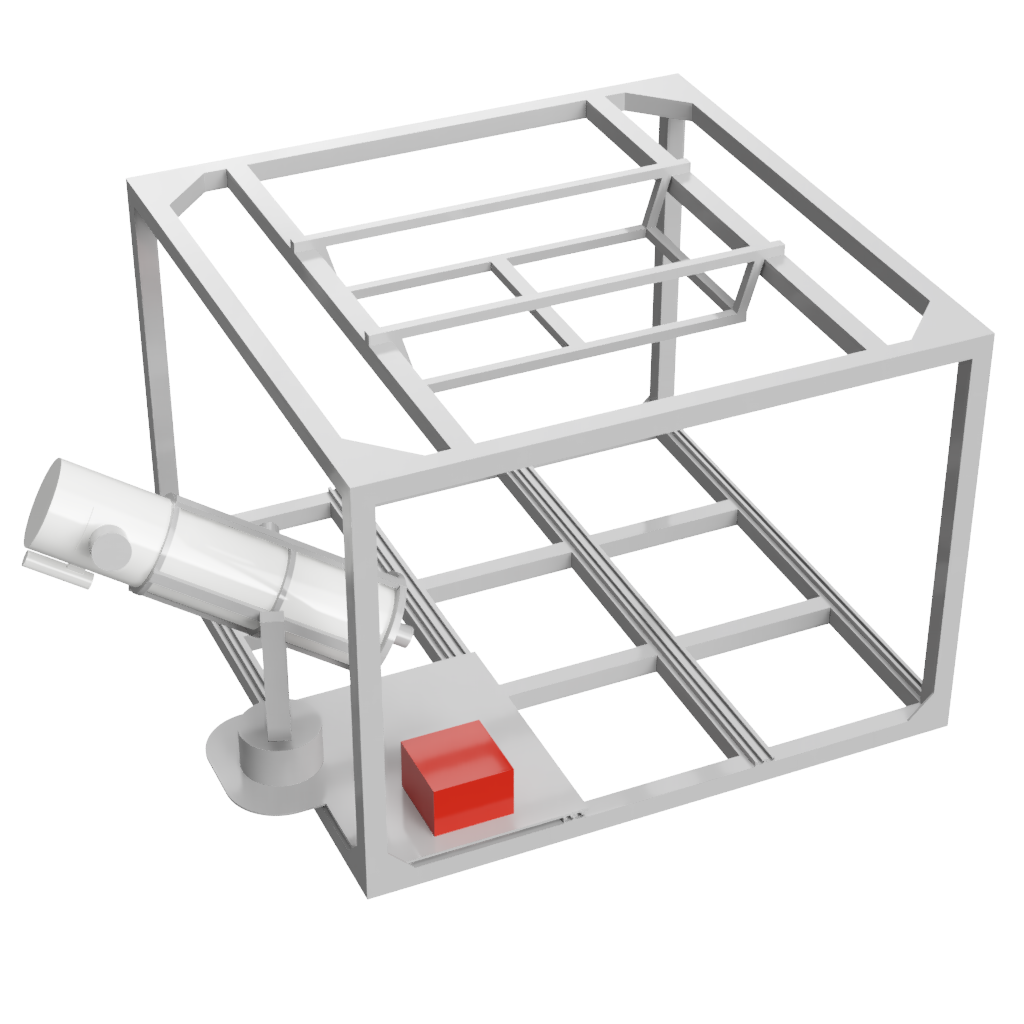
\includegraphics[scale=0.4]{4-experiment-design/img/mechanical/ebox.png}
	\caption{Experiment placement in the gondola.}
	\label{fig::mechanical::ebox}
\end{figure}


\subsubsection{Gimbal}
\label {sec:4.4.3}

The gimbal structure is made from aluminium extrusions with standard fastener brackets, steel rods and sheet aluminium. It is driven by geared stepper motors connected to worm gearboxes. The telescope is held by clamping rings included with the telescope. 

\subsubsection{Transmission}
\begin{figure}[H]
	\centering 
	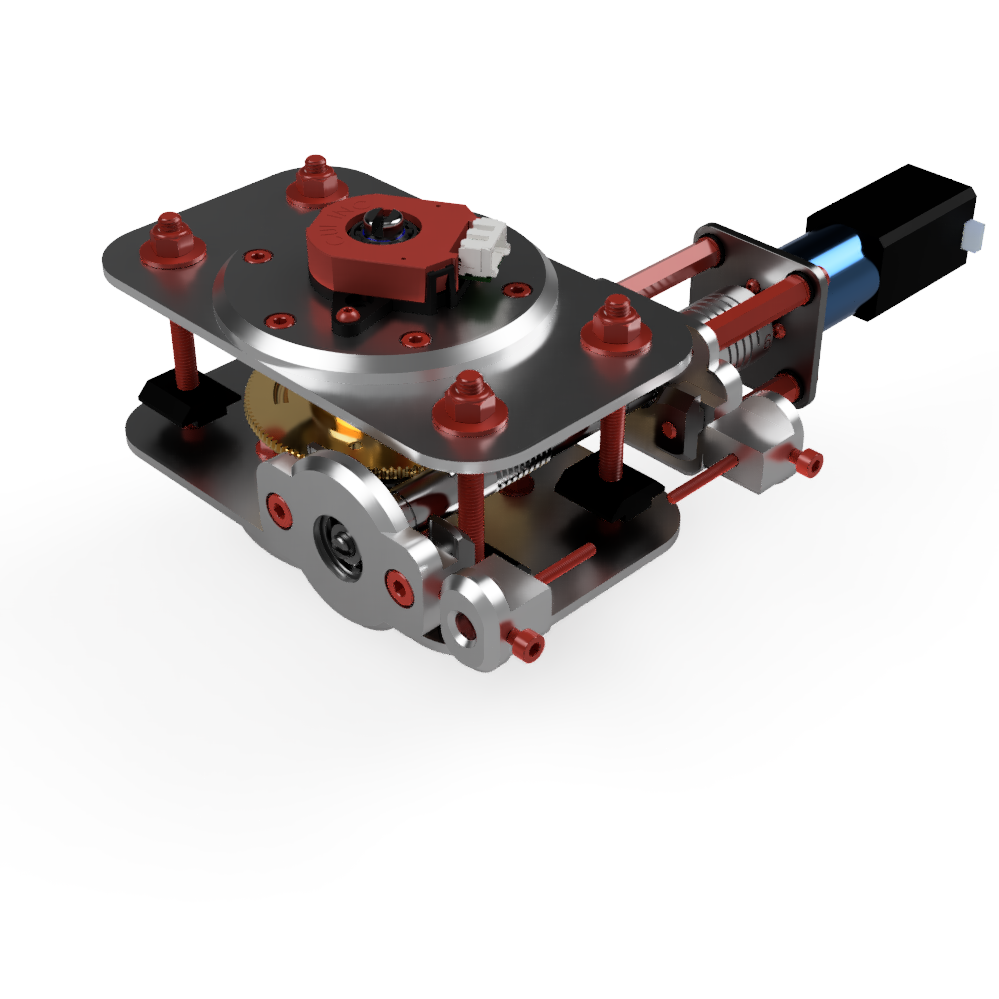
\includegraphics[scale=0.4]{4-experiment-design/img/mechanical/transmission.png}
	\caption{Transmission mechanism. The blue part is the primary planetary gearbox.}
	\label{fig::mechanical::transmission}
\end{figure}

The azimuth and elevation gearboxes are essentially identical, the only difference is the length of the main shaft. The gimbal arm extrusions serve as frames for the worm drives. Holes for the worm wheel and worm shaft are cut and CNC-machined aluminium bearing flanges are attached using bolts and t-slot fittings. Table \ref{tab:mechanical-gearbox} lists the main parameters of the gearbox design. An exploded view is available in Appendix C. \\
% highy recommend https://www.tablesgenerator.com/

\begin{center}
\begin{table}[H]
\begin{tabular}{ll|ll}
Motor holding torque              & 0.07 N & Worm shaft diameter   & 8 mm         \\
Primary gearbox ratio             & 51:1   & Worm shaft bearing    & SKF 708      \\
Primary gearbox efficiency        & 73\%   & Output shaft diameter & 10 mm        \\
Worm drive ratio                  & 58:1   & Output shaft bearing  & SKF 7200  \\
Worm drive efficiency (estimated) & 0.4    & Step resolution       & 2.2 arc sec  \\
Total ratio                       & 2958:1 &                       &             
\end{tabular}
\caption{Gearbox parameters.}
\end{table}
\label{tab:mechanical-gearbox}
\end{center}

The main shaft arrangement is shown in \ref{fig::mechanical::gear_cs}. The bearings are preloaded with conical spring washers, adjusted by shims. The worm wheel is split in two halves and loaded with a torsion spring to make the transmission output essentially backlash-free. The wheel is held by a 3 by 3 mm key that runs through the entire wheel hub. Shaft collars restrict the mechanism axially.

\begin{figure}[H]
	\centering 
	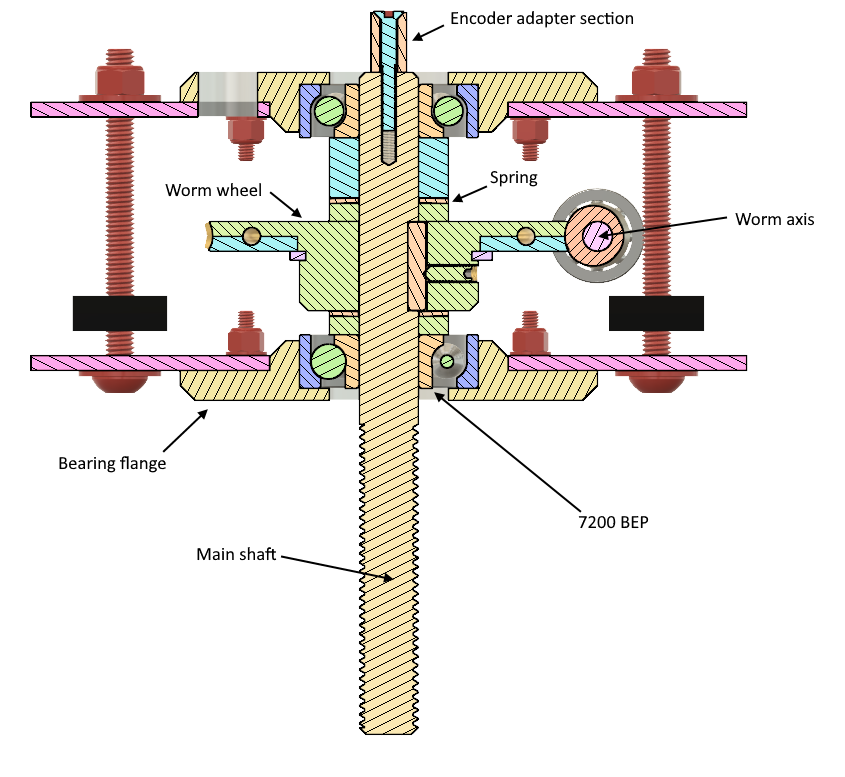
\includegraphics[scale=0.7]{4-experiment-design/img/mechanical/Gearbox_CS.png}
	\caption{Transmission cross-section, front view.}
	\label{fig::mechanical::gear_cs}
\end{figure}

The main shaft arrangement was simulated using SKF SimPro Quick \cite{SKF} and the starting torque was found to be less than 0.3 Nm in the worst case, where the telescope weight is perpendicular to the shaft. This is less than the minimum torque required to turn the backlash mechanism. 

\begin{figure}[H]
	\centering 
	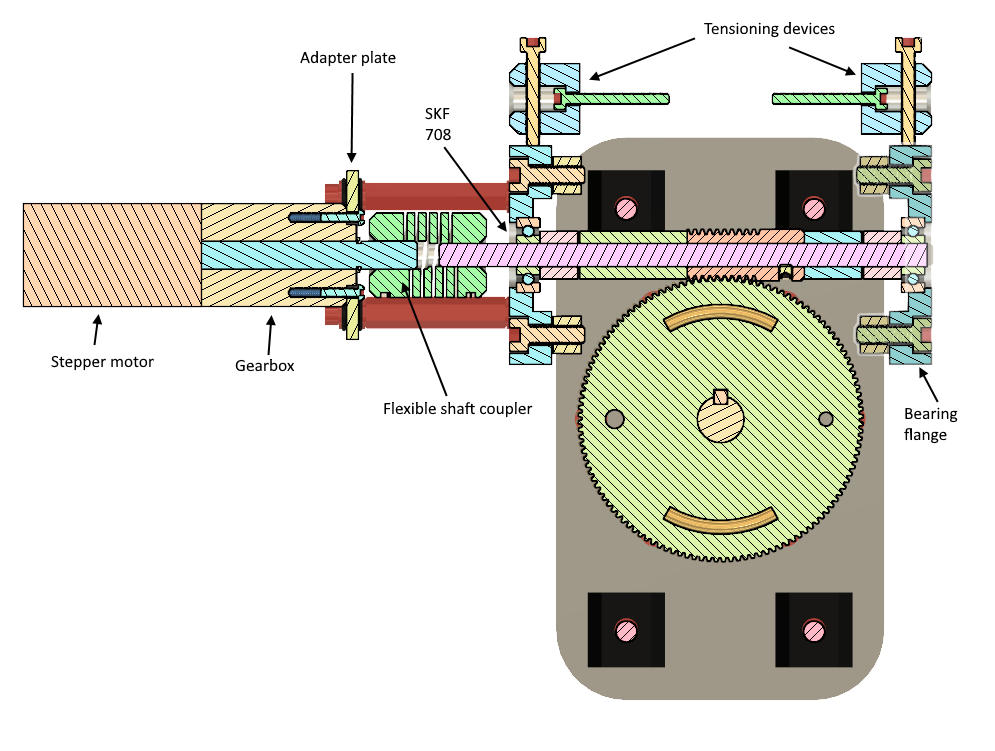
\includegraphics[scale=0.6]{4-experiment-design/img/mechanical/Wormshaft_CS.png}
	\caption{Transmission cross-section, top view.}
	\label{fig::mechanical::worm_cs}
\end{figure}

The worm axis (\ref{fig::mechanical::worm_cs}) uses SKF 708 angular contact bearings preloaded with conical disc springs in an arrangement similar to the main axis. The worm is affixed using two set screws and detents in the worm shaft at 90\degree anglet. The worm shaft pressure can be adjusted using the two tensioning devices. 

The planetary gearbox is coupled to the worm shaft with a flexible shaft coupler, and the entire motor/gearbox assembly is mounted to a steel adapter plate on standoffs. 

\subsection{Field rotator}

The telescope will use an Pyxis LE camera field rotator made by Optec. 

\subsubsection{Moments of inertia and center of mass}

A detailed CAD model of the gimbal structure was made to verify that the center of mass of the telescope can be adjusted such that the side loading on the azimuth axis is minimized. This model was also used to extract estimates for moments of inertia. See Appendix C.

\subsubsection{Safety considerations}

Most parts of the experiment are firmly attached with steel bolts and will not detatch in case of shock. The field rotator and camera are only attached with optical instrument fittings that are not designed for high forces. Therefore the camera and field rotator will have provisions for kevlar safety straps that will be anchored to the telescope mounting ring. 

\subsection{Manufacturing}

The bearing flanges of the transmission and motor adapters/flanges were manufactured using aluminium 60601 with a 3-axis CNC milling machine at the LTU campus in Kiruna.

\begin{figure}[H]
	\centering
	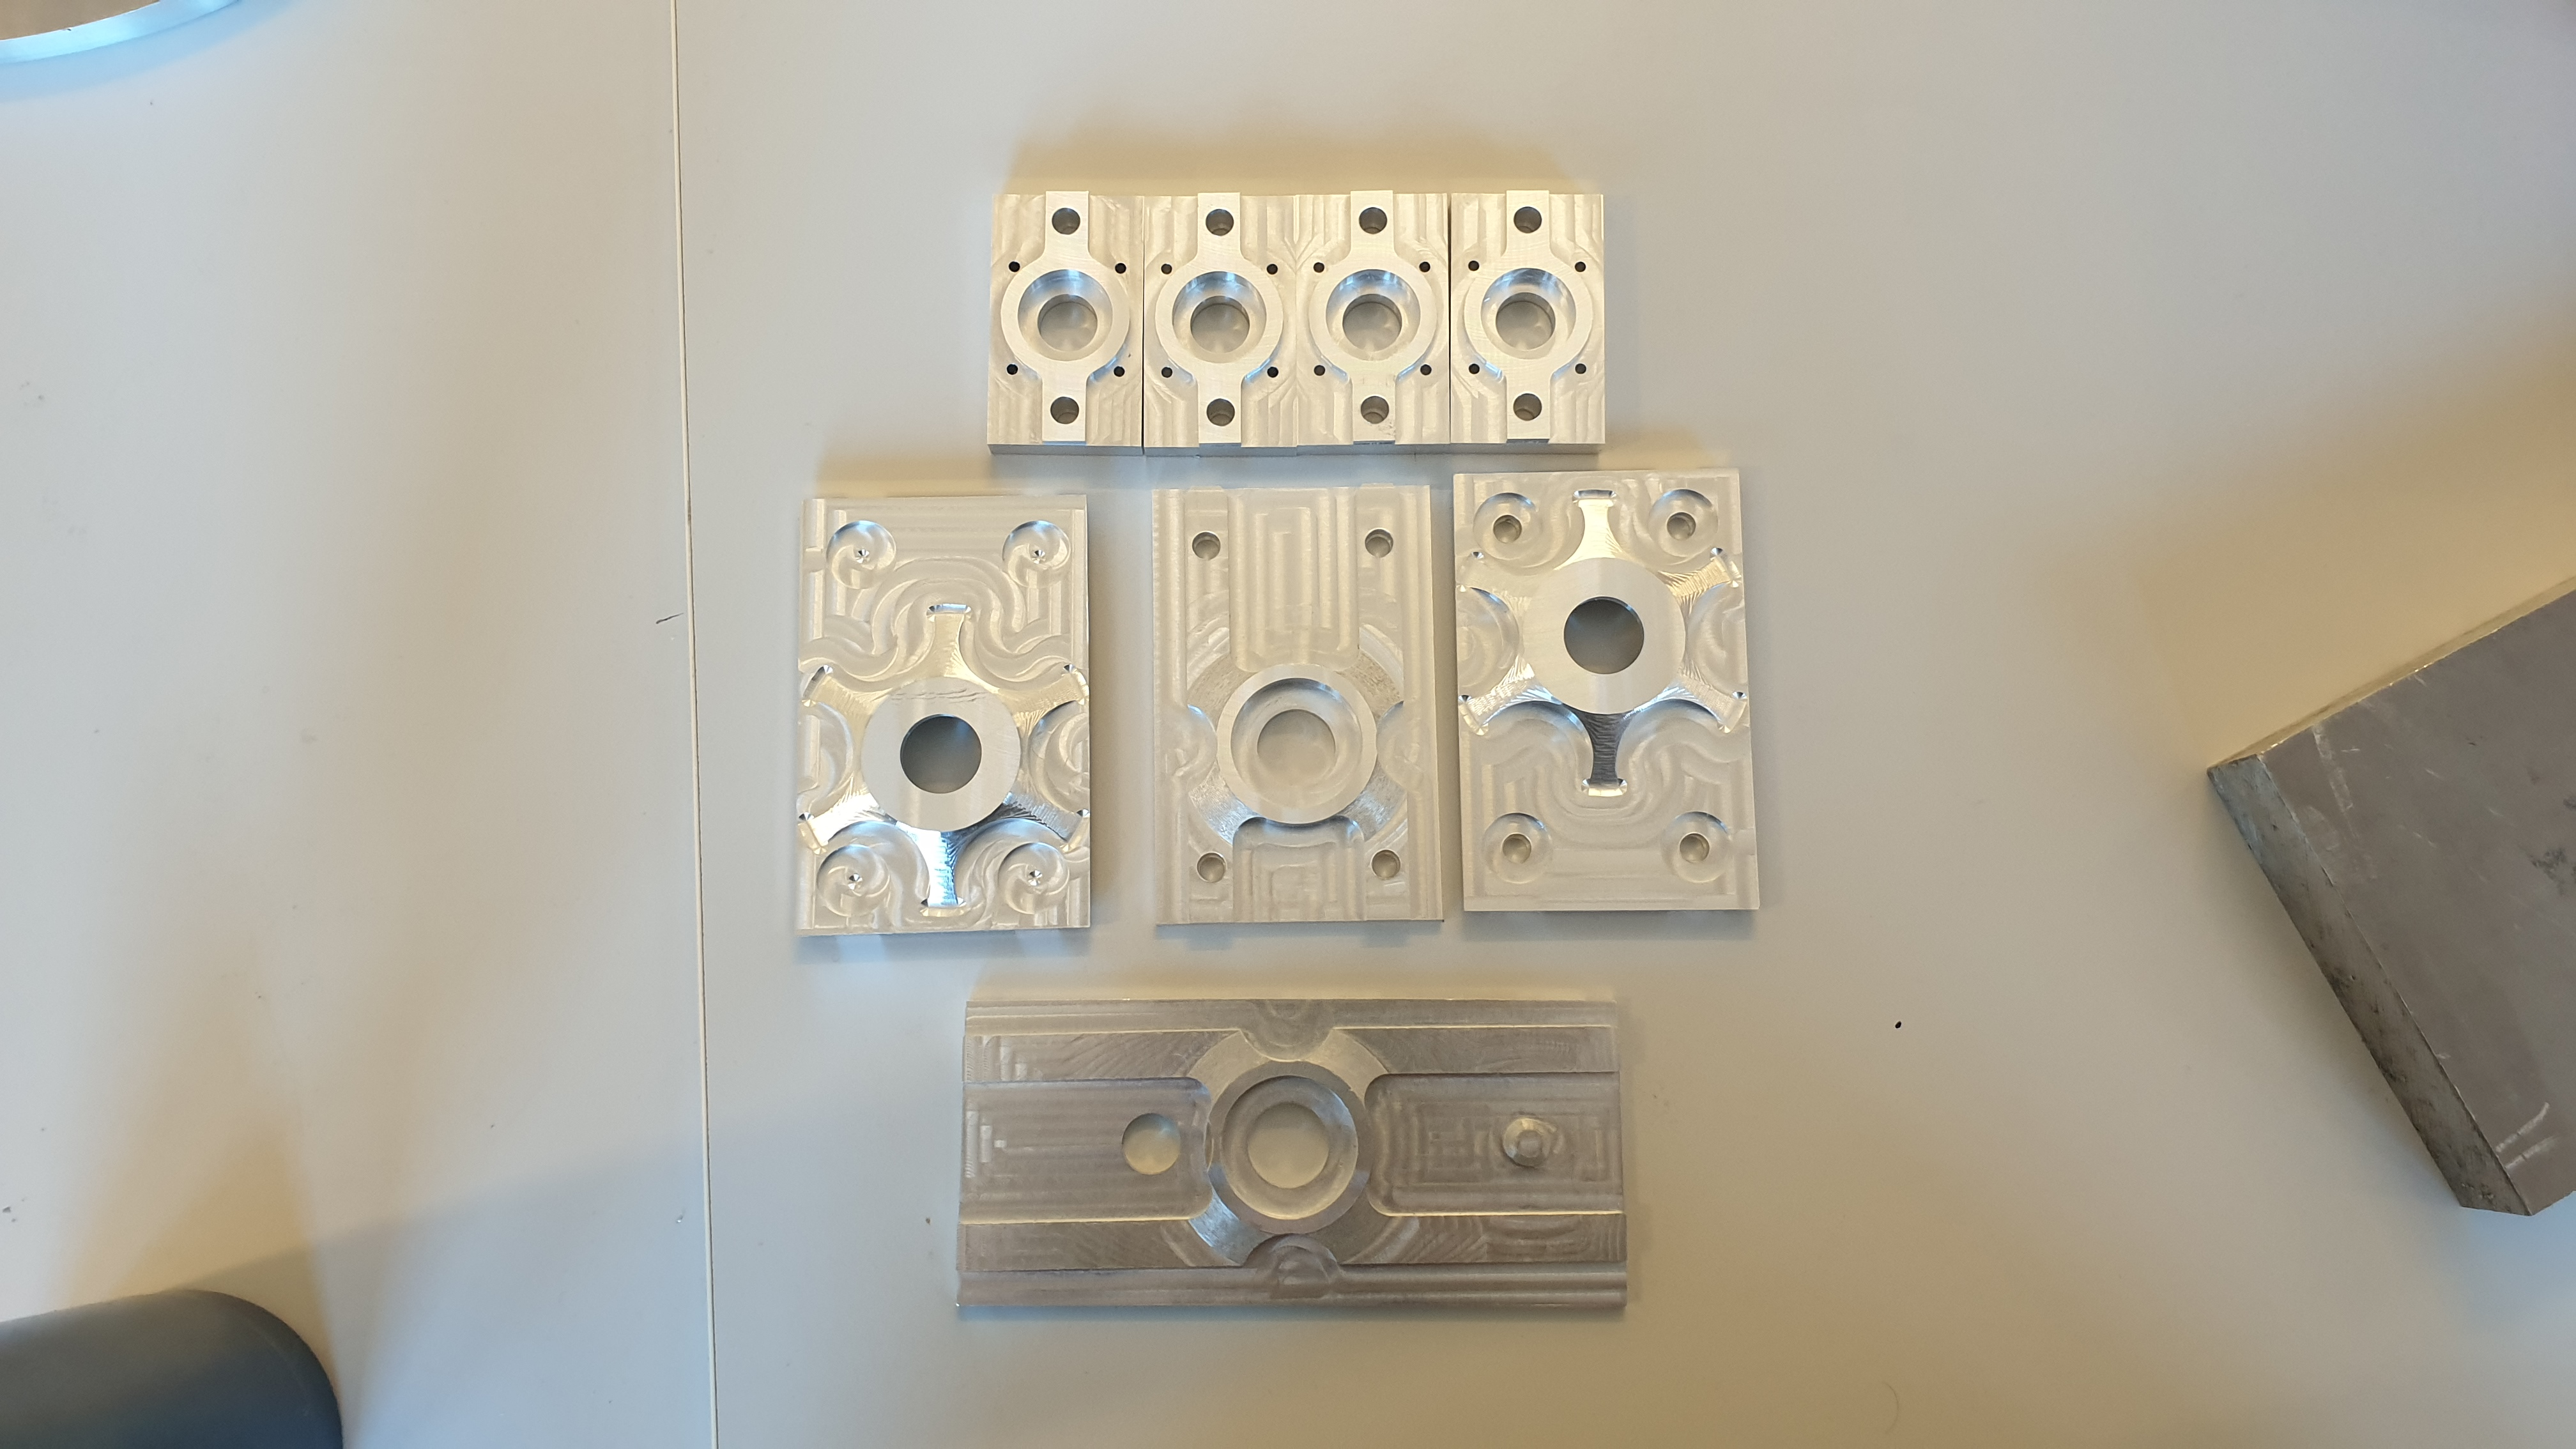
\includegraphics[width=\textwidth]{4-experiment-design/img/mechanical/mach-flanges.jpg}
	\caption{Machined components}
	\label{fig::mechanical::machined_flanges}
\end{figure}

The aluminium extrusions were also machined in order to house the transmissions as shown in some of the drawings, a couple of pictures are shown below:

\begin{figure}[h]
	\centering
	\begin{minipage}[t]{0.4\linewidth}
		\centering
		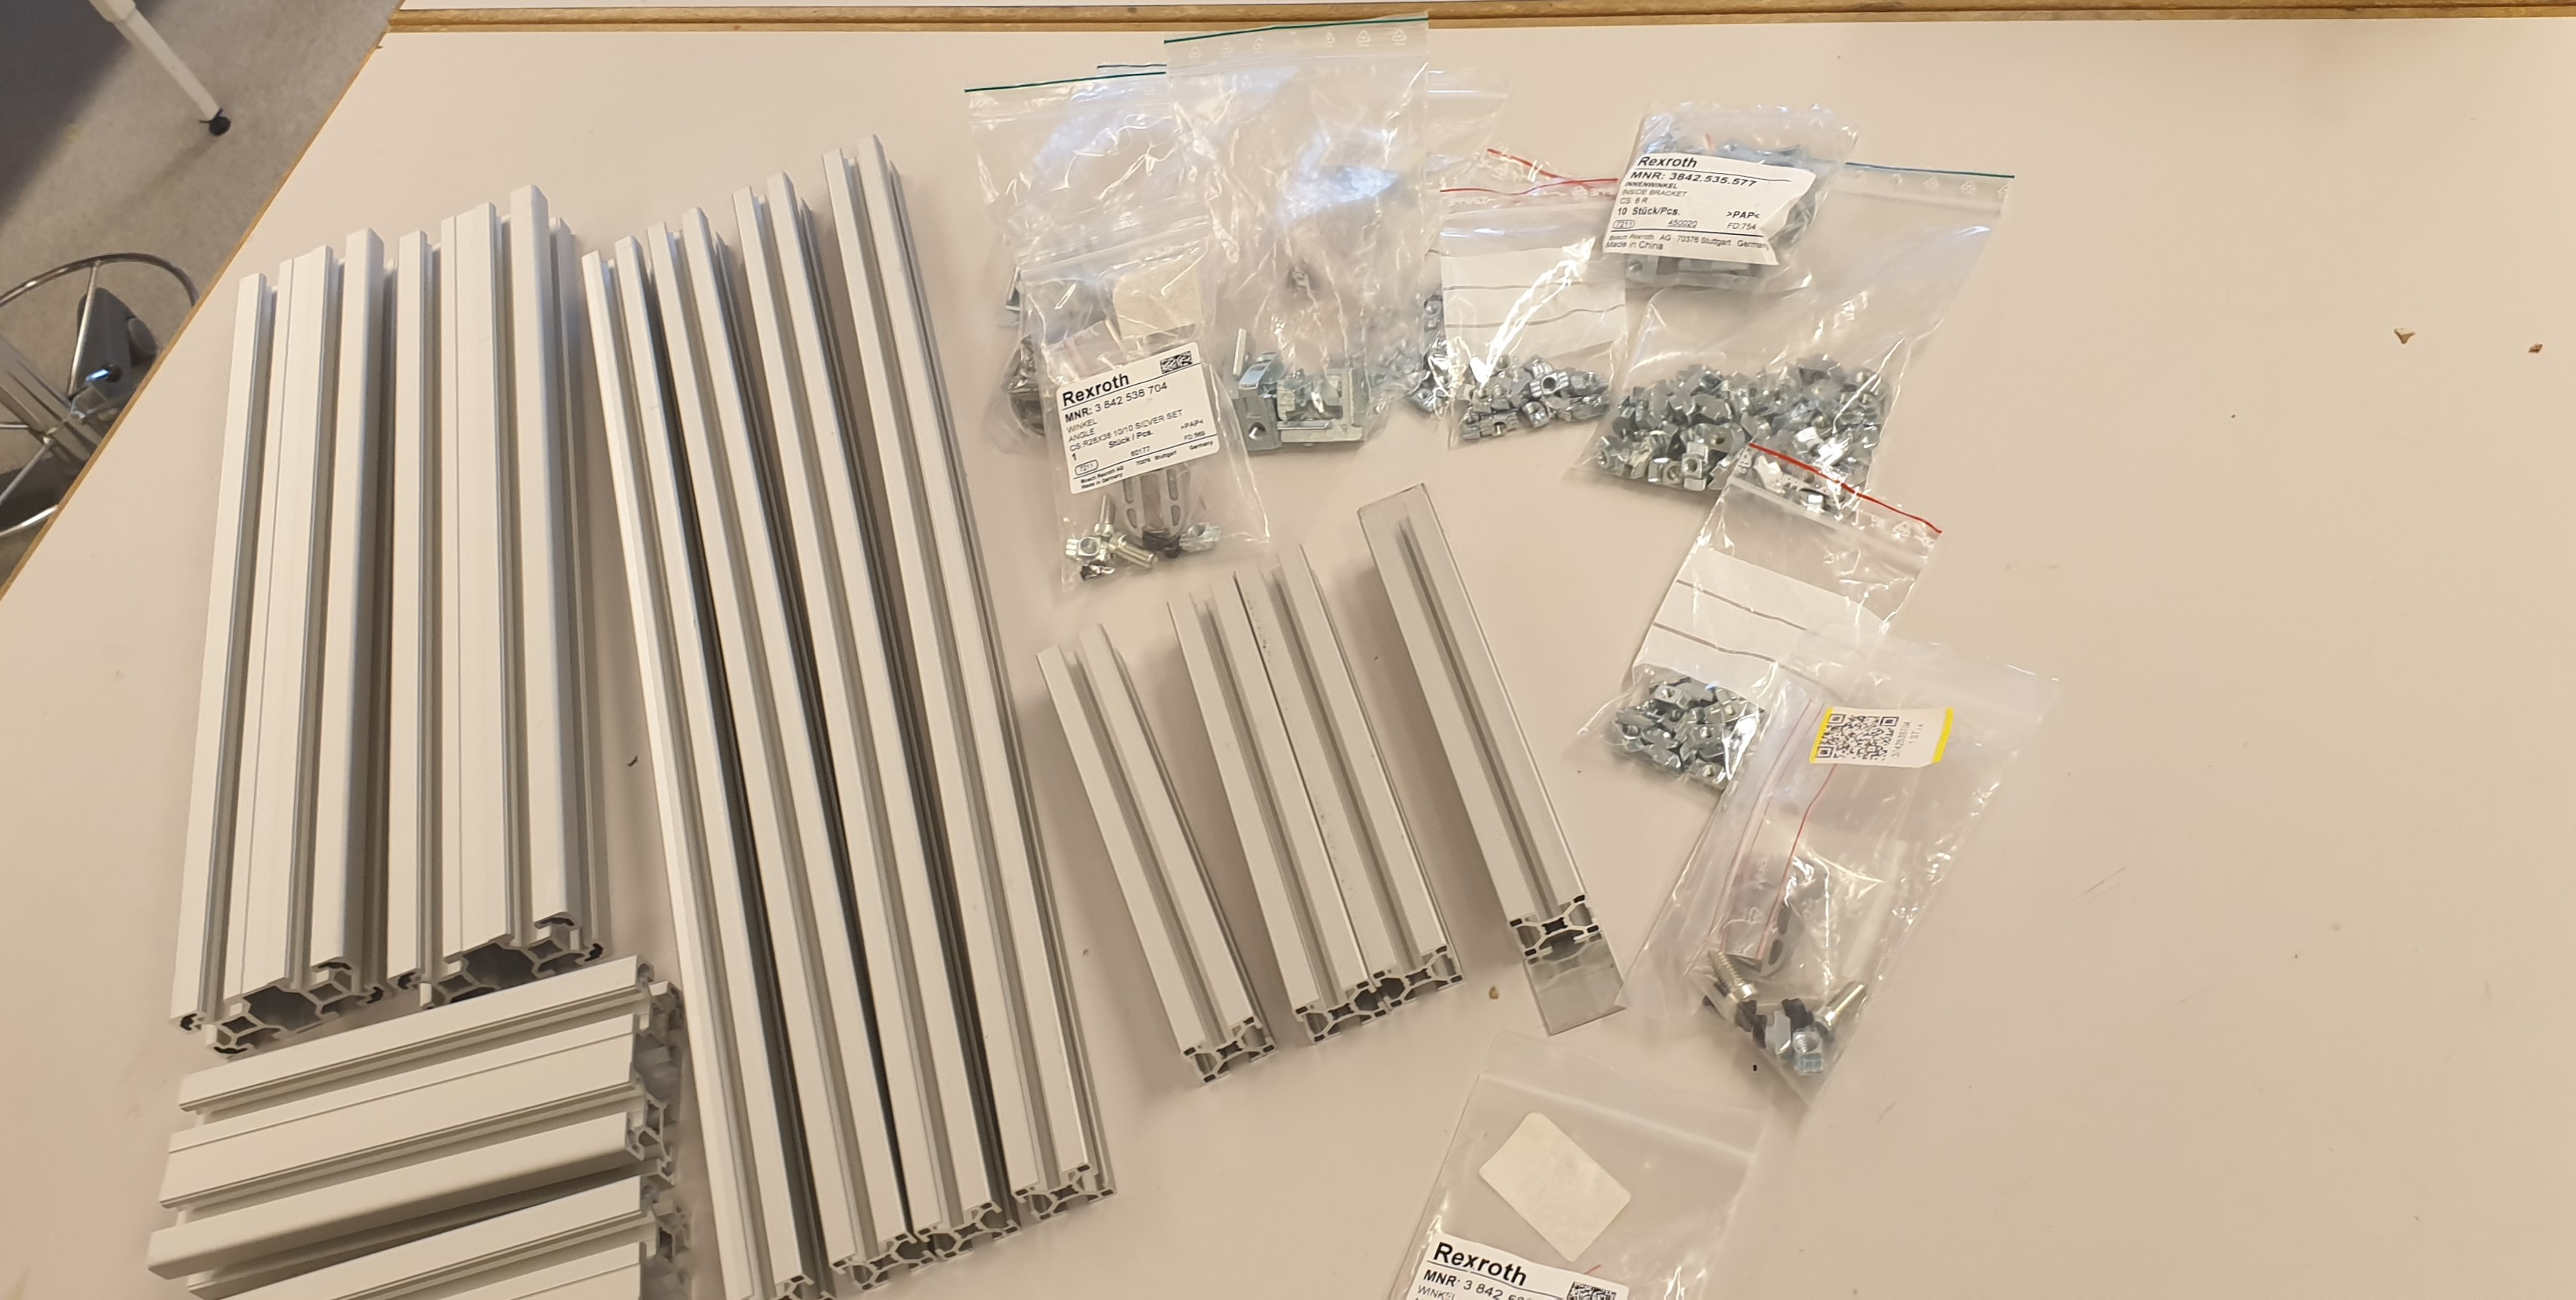
\includegraphics[width=1\linewidth]{4-experiment-design/img/mechanical/extr.jpg}
		\caption{\hl{Aluminium extrusions after unpacking}}
		\label{fig::mechanical::extrusions}
	\end{minipage}
	%\hfill
	\hspace{0.05\linewidth}
	\begin{minipage}[t]{0.4\linewidth}
		\centering
		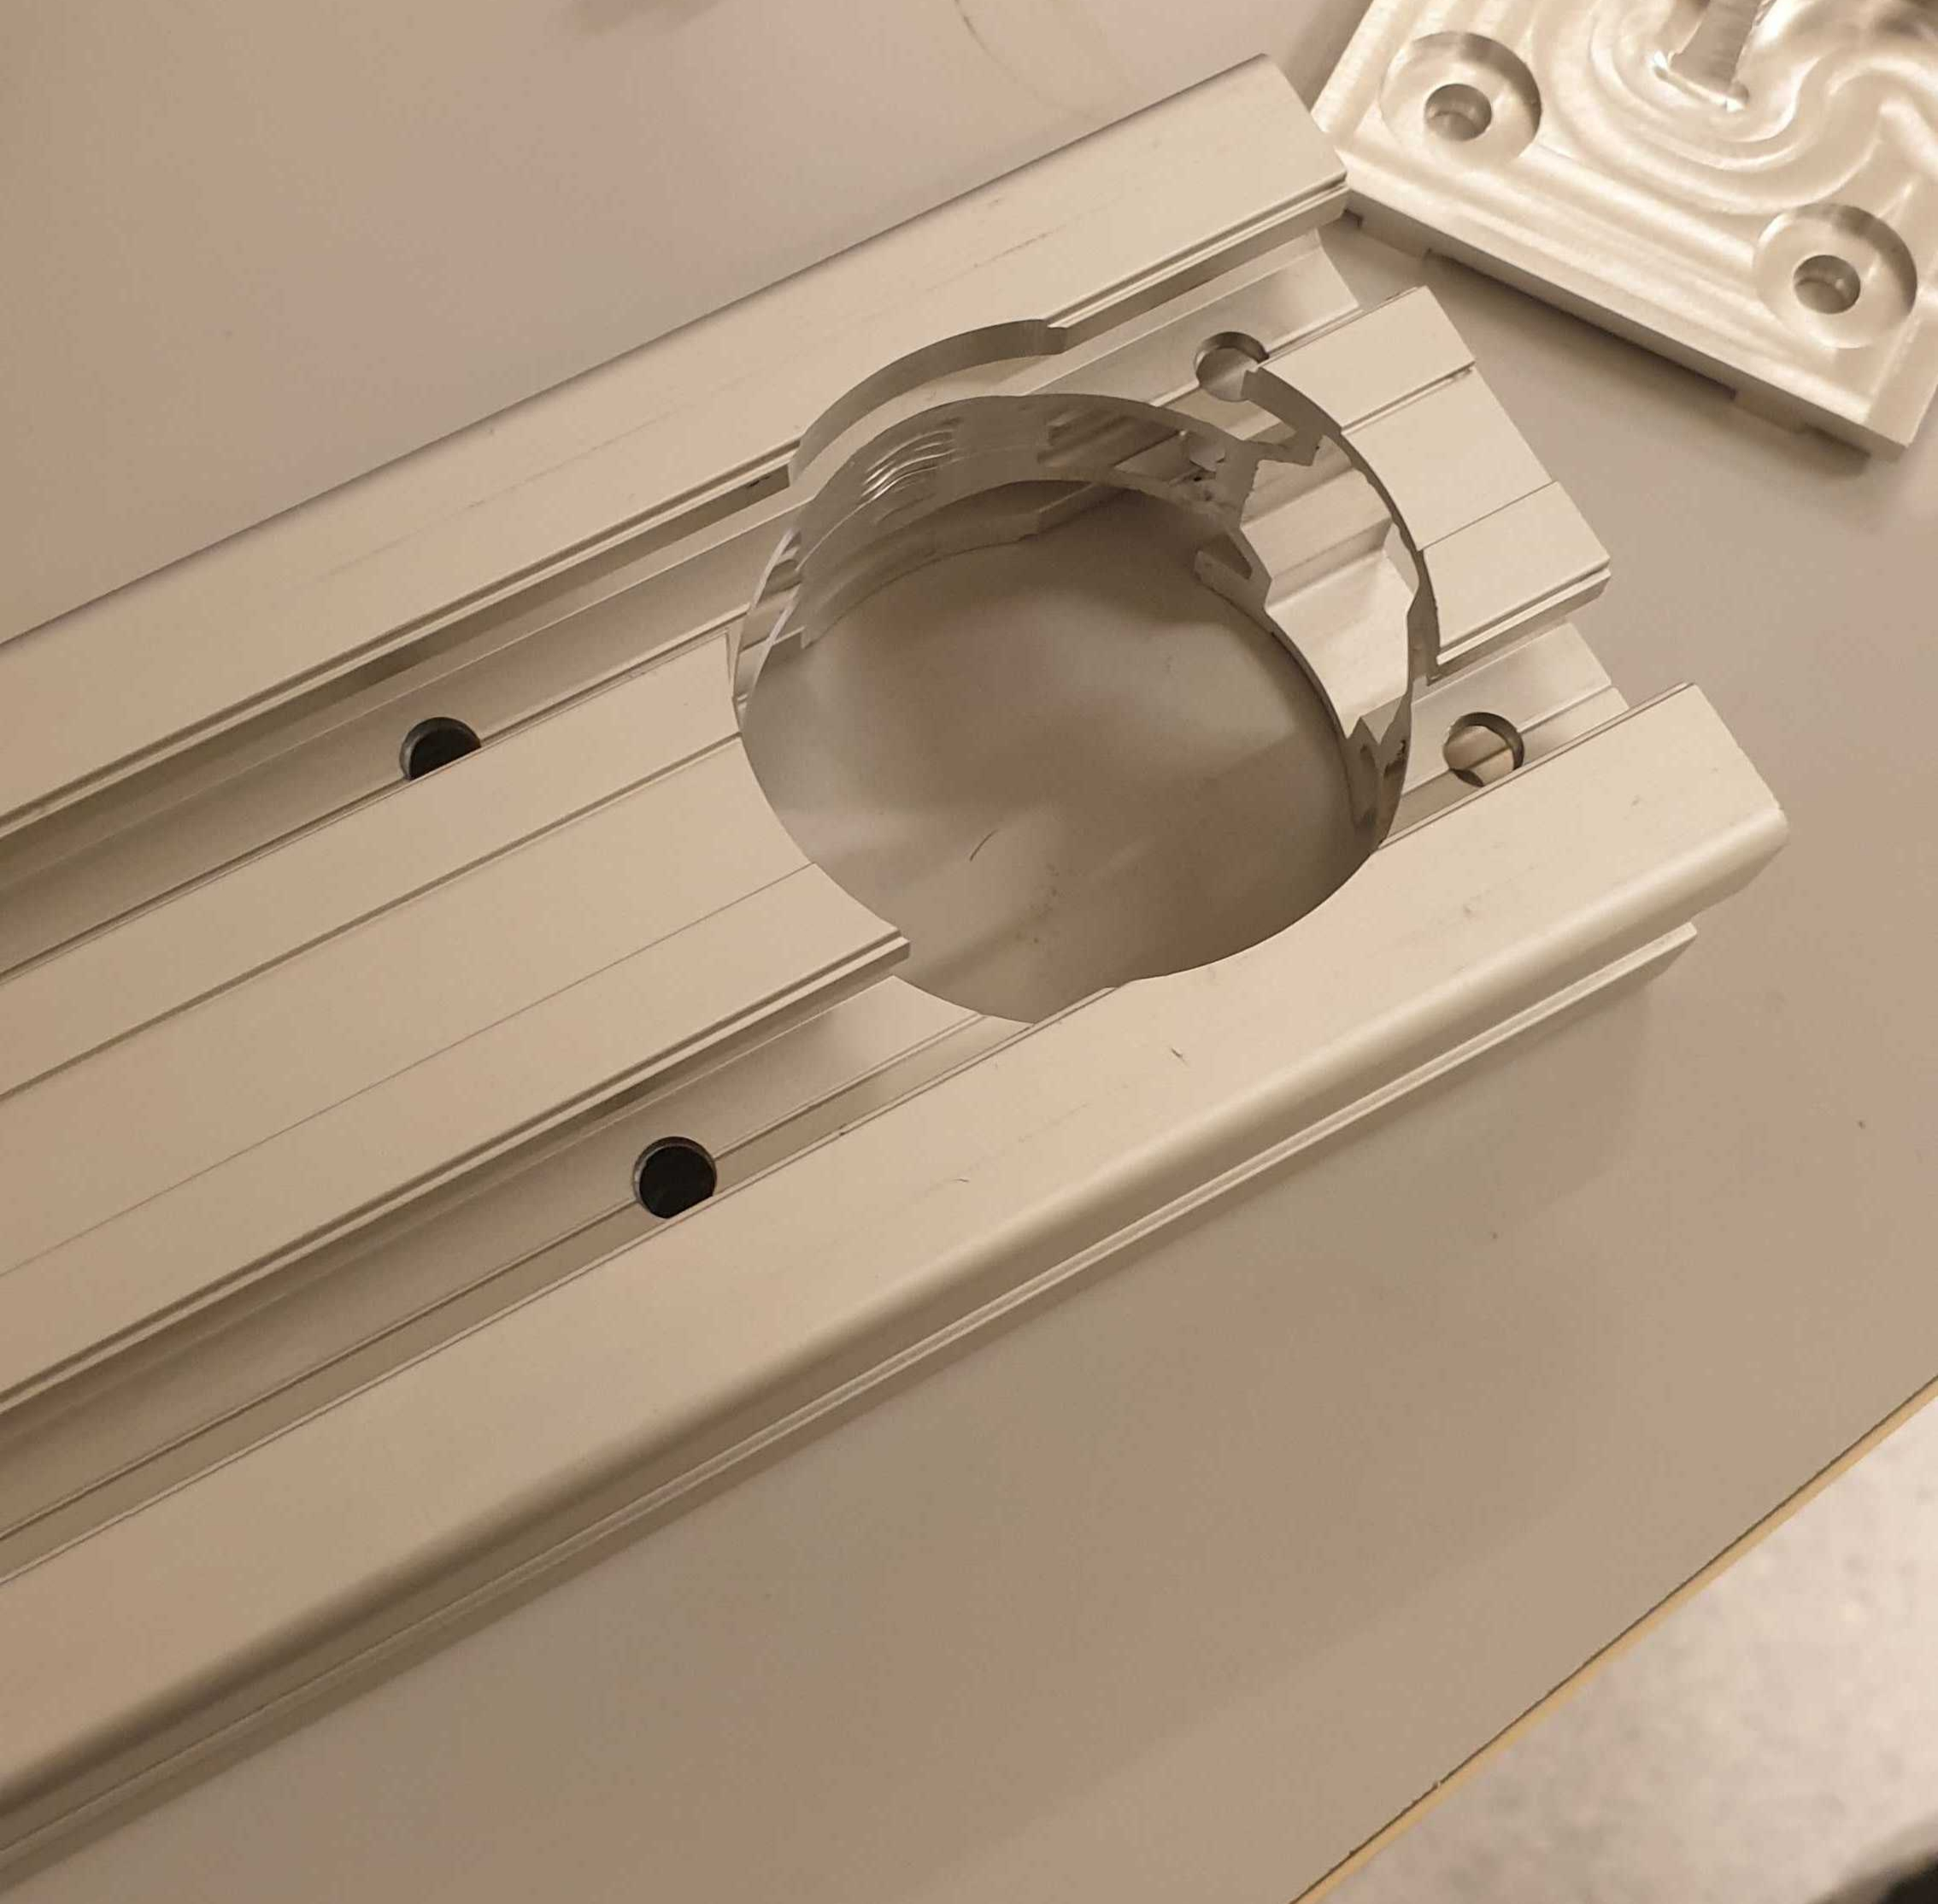
\includegraphics[width=0.65\linewidth]{4-experiment-design/img/mechanical/ext-mach.jpg}
		\caption{\hl{One of the machined extrusions}}
		\label{fig::mechanical::mach-extr}
	\end{minipage}

\end{figure}
